%%=============================================================================
%% Methodologie
%%=============================================================================

\chapter{Methodologie}
\label{ch:methodologie}

%% TODO: Hoe ben je te werk gegaan? Verdeel je onderzoek in grote fasen, en
%% licht in elke fase toe welke stappen je gevolgd hebt. Verantwoord waarom je
%% op deze manier te werk gegaan bent. Je moet kunnen aantonen dat je de best
%% mogelijke manier toegepast hebt om een antwoord te vinden op de
%% onderzoeksvraag.

\section{Redenen van een omschakeling?}
\label{sec:methodologie-redenen-omschakeling}

Puppet is een CMT met vele mogelijkheden maar heeft als nadeel zijn complexe leercurve. Veel mensen waaronder ook \textcite{danAnsiblevsPuppet} en zijn collega's, \textcite{martinAnsiblevsPuppet} en \textcite{AliAnsiblevsPuppet} delen deze mening. Dit was ook het probleem bij de \gls{VRT}. Door de complexiteit waren er maar een beperkt aantal mensen die het volledige potentieel van Puppet konden benutten. Binnen \gls{VRT} was voornamelijk \'e\'en persoon beslagen in Puppet en bovendien was kennisoverdracht naar andere mensen een pijnpunt vanwege drukke agenda's. Dit maakte hem tot een signle point of failure binnen de organistatie.

Door het gebrek aan een goed ingebouwde monitoringstool kost het veel werk om te controleren welke servers correct geconfigureerd zijn. Idealiter zou er  `s ochtends gekeken worden welke servers groen en rood kleuren. Voorlopig gebeurt dit via de command line interface.  

Verder maakt de \gls{VRT}, zoals vele bedrijven, gebruik van meerdere omgevingen. Zo bestaat er van veel servers een versie in development, staging en productie. Op die manier kunnen nieuwe configuraties eerst in de development omgeving uitgetest worden alvorens deze in productie te brengen. Puppet was op de \gls{VRT} niet geoptimaliseerd om het verschil te kennen tussen deze omgevingen. Dit heeft tot gevolg dat Puppet nieuwe configuraties pusht naar elke server, ongeacht of deze productie-kritisch is of niet. Dit is vanzelfsprekend niet de bedoeling en om dit te voorkomen, wordt er momenteel handmatig bepaald welke servers mogen updaten en niet. 
 
Puppet biedt voor veel van deze problemen een oplossing (denk maar aan Puppet dashboard). Doch, mochten veel van deze oplossingen ge\"integreerd worden, dan zou dit leiden tot een  nieuwe refactor van de infrastructuur. Dit, terwijl een refactor in het verleden al tot twee maal toe gebeurd is. Daarom is er besloten om over te schakelen naar Ansible om een zo groot mogelijk draagvlak te cre\"eren. Hoe meer mensen in staat zijn om met Ansible te werken; hoe beter deze \gls{CMT} ge\"integreerd en gebruikt zal worden. Iets wat bij Puppet niet mogelijk is vanwege de complexiteit.

Ansible biedt met Ansible Tower een ge\"integreerde monitoringstool. Bovendien wordt deze \gls{CMT} door velen geprezen vanwege zijn eenvoud in syntax. Ook de opstelling van de infrastructuur is eenvoudiger. Zo heeft Ansible geen agent nodig om servers te configureren wat een enorm voordeel biedt. Er kan dus zonder iets te moeten installeren onmiddellijk overgegaan worden tot het configureren van clients. Ansible Tower kan met vele externe technologie\"en overweg wat de mogelijkheden tot continuous deployment vereenvoudigt. Zo is bijvoorbeeld git ingebouwd wat zorgt voor een eenvoudig beheer van de source code.

%TO DO - hoe eenvoudig ansible is om te leren
%- slechte monitoring
%- slecht geautomatiseert 
%- geen multi environment
%- expert vertrokken
%- gui veel werk en complex
%- oorspronkelijk geen modules, refactor, in feite nu weer refactor
%- updates zorgen voor compatiblieteistproblemen (denk ik)
%- puppet client niet ouder dan puppet master maar omgekeerd denkik wel (op te zoeken)

\section{Werking van Ansible en Puppet}
\label{sec:methodologie-technische-verschillen}

\subsection{Overzicht van Puppet en Ansible}



\begin{minipage}{15cm}
\begin{tabular}{ r |c c }
& \textbf{Ansible} & \textbf{Puppet} \\
  \hline	  		
\gls{programmeerparadigma}  & declaratief & declaratief  \\
\hline
Geschreven in & YAML & \gls{dsl}  \\
\hline
Gebasseerd op & Python & Ruby \\
\hline
Communicatieprotocol & SSH & HTTPS \\

\hline
  Push / Pull principe \footnote{Beide technologie\"en zijn in staat om zowel volgens push als pull methode te functioneren. Zo heeft Ansible ‘pull-mode' \autocite{ansiblePull} en \textcite{puppetkick} ‘Puppet kick' } & \gls{push} & \gls{pull} \\
   \hline
   open poorten\footnote{Dit zijn de minimale vereisten van open poorten. Voor sommige features dienen meer poorten open te staan. Bijvoorbeeld 443 voor Ansible Tower of 8140 op elke Puppetclient voor de Puppet kick functionaliteit \autocite{puppetkick} }  & 22/tcp (client) & 8140/tcp (master)\\
  \end{tabular}
  \end{minipage}   

 Informatie opgehaald van \textcite{languagePuppet}, \textcite{masterproef}, \textcite{ansibledoc}



\subsection{Werking van Puppet}

Tussen de master en de client bestaat er een vertrouwensrelatie die onderhouden wordt door certificaten. Het is de Puppetmaster die verantwoordelijk is voor het verlenen van deze certificaten. Pas als deze in orde zijn kan Puppet  aan de configuraties van de clients beginnen. De verzameling van alle geschreven code wordt een manifest genoemd. Wanneer een Puppetagent wil controleren of hij nog up-to-date is, zal hij een catalogus aanvragen bij de Puppetmaster. Een dergelijke catalogus is in feite een manifest dat de Puppetmaster compileert. Deze catalogus is bovendien uniek voor elke Puppetagent. Dit komt omdat er bij het compileren van het manifest naar de catalogus rekening gehouden wordt met diverse parameters zoals de functie van de server of de distributie van het besturingssysteem dat op die server draait \autocite{Puppetlanguagecatalog}. Eens de Puppetagent zijn persoonlijke catalogus ontvangen heeft, zal deze voor zichzelf controleren of er verschillen zijn tussen zijn huidige configuratie en de staat die beschreven staat in de catalogus. Indien er afwijkingen zijn, worden deze ook automatisch opgelost \autocite{puppetdoc}.

\begin{figure}  \begin{center}
  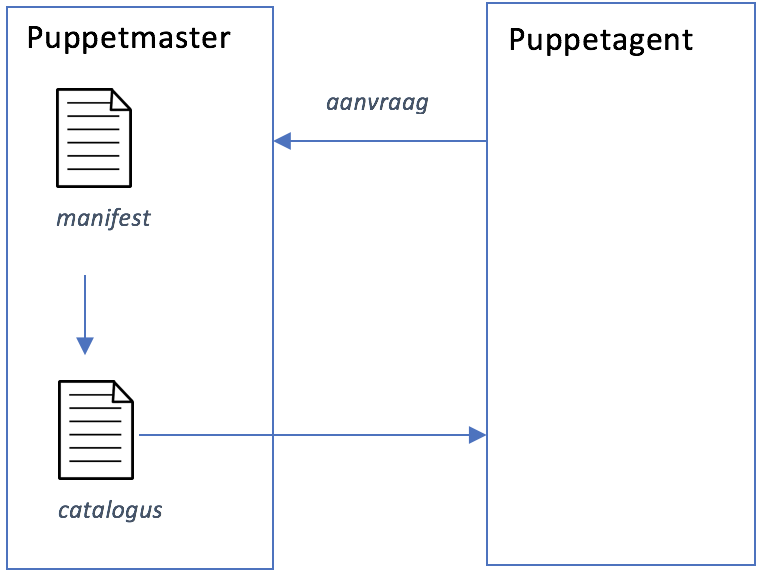
\includegraphics[width=250px]{img/aanvraagCatalogus.png}
 \end{center}\caption{Aanvraag van een catalogus bij de Puppetmaster door een Puppetclient. De Puppetagent is een daemon (stukje software) die op de Puppetclient draait.}  
  \label{fig:aanvraagCatalogus}
\end{figure}


\subsection{Werking van Ansible}

In tegenstelling tot Puppet maakt Ansible geen gebruik van zogenaamde agents. Dit betekent dat de Ansibleserver enkel de naam en het wachtwoord dient te kennen van de servers die hij moet configureren. Het authenticeren kan op verschillende manieren. Er wordt aangeraden om gebruik te maken van een SSH-key, wat het eenvoudigst is, maar ook andere middelen zoals een eenvoudig wachtwoord of het Kerberos-protocol worden ondersteund. De gewenste configuraties worden geschreven in playbooks met bijhorende Ansiblerollen. Eens een verbinding tot stand is gebracht, wordt het gecompileerde playbook naar de te configureren server gestruurd. Deze worden vervolgens op de clients uitgevoerd  en weer verwijderd. Ook Ansible bezit de functionaliteit om na te gaan of de huidige configuratie in lijn is met de ontvangen modules. Om servers te configureren met Ansible bestaan er bovendien twee manieren. Ansible playbooks kunnen in principe verstuurd worden naar de servers vanaf elke computer. Voor een grotere hoeveelheid servers is dit echter moeilijk onderhoudbaar en onoverzichtelijk. Hiervoor bestaat er de commerci\"ele versie waarbij de playbooks verstuurd worden vanaf een centraal punt. Dit centraal punt wordt Ansible Tower genoemd; die heeft een inventaris van alle servers en playbooks die onder zijn verantwoordelijkheid vallen. Verschillende gebruikers kunnen vervolgens verschillende toegangsrechten krijgen zodat personen enkel servers kunnen configureren die onder hun bevoegdheid vallen \autocite{ansibledoc}.

%------------------------------------

\section{Technische analyse van Ansible en Puppet}
\label{sec:technischeanalyse}
\subsection{Opstelling van de testomgeving}
\label{sec:opstellingtestevn}
\subsubsection{Architectuur van de opstelling}

%\begin{wrapfigure}{R}{0.4\textwidth}
%	\centering
%	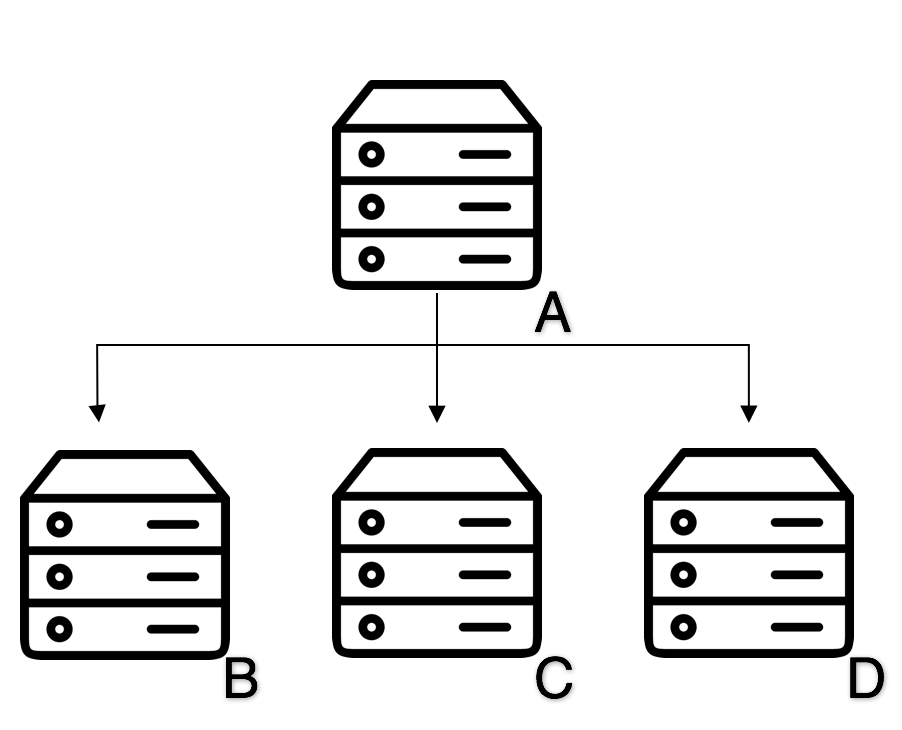
\includegraphics[width=0.4\textwidth]{img/infrastructruur.png}
%	\caption{\label{fig:infrastructuur} Server A, de master, configureert server B - D, de clients.}
%\end{wrapfigure}

\begin{wrapfigure}{R}{0.25\textwidth}
	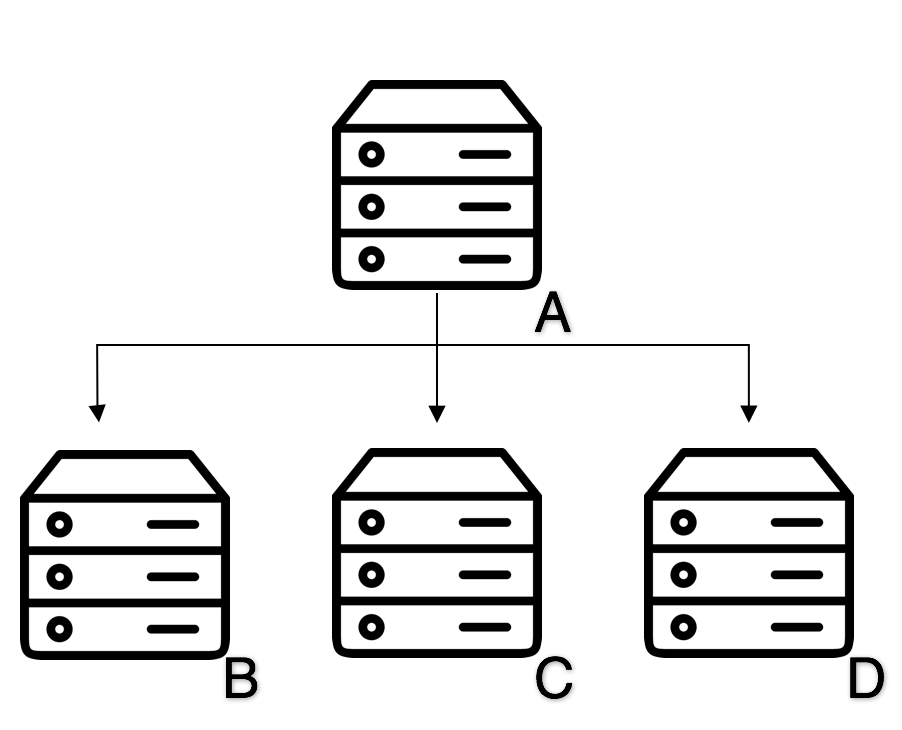
\includegraphics[width=0.9\linewidth]{img/infrastructruur.png} 
	\caption{Server A is de master en configureert clients B tot D.}
	\label{fig:infrastructuur}
\end{wrapfigure}

%Vagrant is a tool for building and managing virtual machine environments in a single workflow

Deze opstelling is gerealiseerd door gebruik te maken van \textcite{whatisvagrant}. Dit is een tool die het mogelijk maakt om op eenvoudige wijze meerdere virtuele omgevingen op te zetten, te configureren en te beheren.  Voor elke omgeving bestaat er een Vagrantbestand. Er is dus een Vagrantbestand voor de Ansibleinfrastructuur en \'e\'en voor de Puppetinfrastructuur. Voor elk van deze omgevingen wordt eerst de master aangemaakt, gevolgd door een X-aantal clients. Vagrant zorgt ervoor dat elke client  verbonden wordt met New Relic. Dit is de gekozen tool om de servers te monitoren. In het geval van Puppet wordt hierbij ook nog de Puppetagent ge\"installeerd. Elke client, zowel in de Ansible- als de Puppetinfrastructuur, is gebaseerd op dezelfde basebox en krijgt dezelfde resources toegekend. De masters beschikten over meer resources.

\fbox{\begin{minipage}{15em}
\textbf{Technische specificaties clients}\newline
Basebox: bertvv/centos72\newline
Aantal CPU's: 1\newline
Geheugen: 500 MB
\end{minipage}}

\subsubsection{Modus operandi}

Elke server wordt opgezet door middel van Vagrant. De situatie vlak nadat Vagrant de servers opgezet heeft, wordt hierna de ‘beginstand' genoemd.
Vanuit deze situatie nemen de \gls{CMT}'s het over. Afhankelijk van de test worden de resultaten afgelezen van ofwel de \gls{CMT} ofwel de monitoringstool. 
Elke test wordt 30 keer uitgevoerd. Telkens de test opnieuw wordt uitgevoerd, wordt deze eerst terug naar de beginstand gebracht\footnote{Weliswaar is deze beginstand voor de testen van ‘\gls{partialconfig}' en ‘geen configuratie' verschillend.}.
Deze gegevens worden vervolgens afgelezen en in een tabel genoteerd. Deze ruwe data wordt achteraf opgeschoont\footnote{Zo worden gegevens die geen onderdeel meer uitmaakten van de test verwijderd of werd er gezorgd dat elke dataset even lang is. Belangrijk is te weten dat deze aanpassingen enkel gebeurd zijn waar mogelijk en dat deze geen invloed hebben op berekeningen en conclusies. } en kan teruggevonden worden in bijlage C, datasets. Achteraf is het op deze data dat de analyses en mathematische berekingen zijn gebeurd. De conclusies kunnen teruggevonden worden in onderstaande secties.

\subsubsection{Configuratie van servers door CMT's }


Voor de testen in sectie \ref{sec:technischeanalyse} is er gekozen om gebruik te maken van een LAMP-stack. Dit is zowel voor Ansible als Puppet gebeurd. Bovendien werd er getracht om in de mate van het mogelijke beide configuraties zo analoog mogelijk te houden. Om dit te realiseren wordt er httpd, php, php-mysql en mariaDB ge\"installeerd op de servers. Vervolgens wordt er een webpagina op de site geplaatst. Deze is geschreven in PHP en controleert of alle zaken naar behoren werken. Om af te sluiten wordt HTTP doorgelaten door de firewall, de service httpd gestart en MariaDB gestopt. 

Opmerking: De reden dat MariaDB op dit moment nog niet gestart wordt is vanwege de testen bij ‘\gls{partialconfig}'. Hierbij wordt gemeten hoelang het duurt om bij een bestaande configuratie enkele aanpassingen door te voeren. Het is dus pas bij deze testen dat MariaDB gestart wordt.


Deze configuraties kunnen teruggevonden worden op Github op de volgende links\footnote{Mogelijk komt de beschreven configuratie in dit rapport niet volledig overeen met de code op Github. Deze repositories worden namelijk ook gebruikt voor andere testen  binnen dit onderzoek.}:\newline
\textbf{Ansible:} https://github.com/ThomasDetemmerman/AnsibleTower \newline
\textbf{Puppet:} https://github.com/ThomasDetemmerman/PuppetMaster



\subsection{Belasting van het netwerk}
Ansible en Puppet hebben een groot verschil in de manier van communiceren en dit weerspiegelt zich in het gedrag van de \gls{CMT}. De grafieken op afbeeldingen \ref{fig:deploytypes} en \ref{fig:netwerkverbruik} weerspiegelen uitsluitend het dataverkeer tussen de server (Ansible Tower of Puppetmaster) en de desbetreffende client. Andere data zoals bijvoorbeeld het downloaden van services of uploaden van logbestanden naar de monitoringstool zijn hierin \underline{niet} opgenomen. Dit wordt verwezenlijkt door gebruik te maken van verschillende netwerkkaarten. Wanneer er geen deploy gebeurt, is de kilobyte/ minuut op deze netwerkkaart gelijk aan nul; een bewijs dat hier geen andere data dan deze van de \gls{CMT} over wordt verstuurd.  
	
De manier van communicatie is te herkennen in de grafieken. Zo onderhoudt Ansible de communicatie met de client gedurende de \gls{deploy}. Hiermee wordt bedoeld dat Ansible op de hoogte is van de laatste stand van zaken op de client. Wanneer een bepaalde taak voltooid is, wordt Ansibel Tower hier onmiddellijk van op de hoogte gebracht. Zoals te zien is op grafiek \ref{fig:deploytypes} is er geregeld communicatie tussen beide servers. Weliswaar is er enkel communicatie wanneer iets voltooid is; er is dus geen onnodige communicatie. Zo is ook te zien hoe op T5 de communicatie nul is. Ansible had voor die periode niets te melden\footnote{Hier betreft het de service MariaDB die wordt gedownload.}. 

Deze manier van werken is handig tijdens het testen van nieuwe Ansible rollen. Je krijgt namelijk live feedback tijdens het uittesten. Een nadeel is wel dat het netwerk geen rust krijgt. Bovendien wordt deze functionaliteit van ‘live feedback' enkel gebruikt voor testen. Eens een rol operationeel is, loopt deze doorgaans tijdens de nacht en is het voldoende om de dag daarna een algemeen overzicht te krijgen. 

Bij Puppet is dit anders. Hierbij is er enkel communicatie tussen de master en de client bij het begin en op einde van de \gls{deploy}.  Tijdens de eerste reeks vraagt de client een \gls{catalog} op bij de master. Vervolgens worden eventuele \gls{puppetplugin}'s gesynchroniseerd en vraagt de master \gls{fact}s op bij de client. Op basis van deze gegevens wordt uiteindelijk de verwachte \gls{catalog} verstuurd. Tijdens het configureren is er geen communicatie tussen beide servers. Op het einde wordt een rapport in JSON-formaat terug naar de master gekoppeld \autocite{neworkusage}.
 
Een nadeel aan het feit dat er enkel in het begin en op het einde communicatie is, is dat er op de master geen live feedback gevolgd kan worden. Dit kan echter wel opgelost worden door in te loggen op de desbetreffende client en hier de live feedback te volgen met behulp van het commando "\texttt{puppet agent -t}". Het wordt wel nog steeds pas op het einde van de \gls{deploy} terug naar de master gestuurd.

Vervolgens is er ook gekeken naar de totale netwerkbelasting. Hiervoor is er per client een cumulatie genomen van de kilobytes/minuut gedurende de gehele \gls{deploy}. Deze waarden zijn terug te vinden in grafiek \ref{fig:netwerkverbruik}. Hier heeft Ansible een gemiddelde van 5802,29 kilobytes/deploy. Dit terwijl Puppet gemiddeld 9464,32 kilobytes/deploy haalt. 

\textbf{We kunnen dus concluderen dat Ansible minder grote bestanden verstuurt over het netwerk door deze op te splitsen in meerdere kleine bestanden verspreid over de hele \gls{deploy}. Hierbij is wel een voortdurende verbinding vereist tussen beide servers.  Puppet aan de andere kant weet de communicatie te beperken tot twee reeksen. Op het einde van de rit heeft Puppet wel meer bestanden uitgewisseld dan Ansible. }

\begin{figure}
	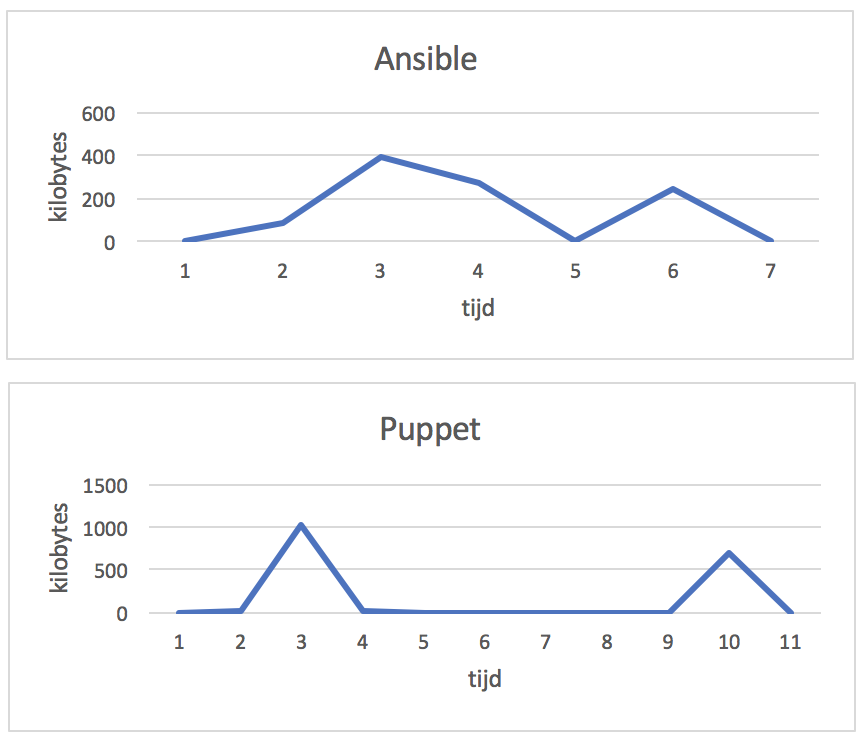
\includegraphics[width=430px]{img/deploytypes.png}
	\caption{Twee manieren van communiceren. Aantal kilobytes per tijdseenheid op een netwerkkaart die uitsluitend bedoeld is voor communicatie met Ansible Tower / Puppetmaster. }  
	\label{fig:deploytypes}
\end{figure}

\begin{figure}
	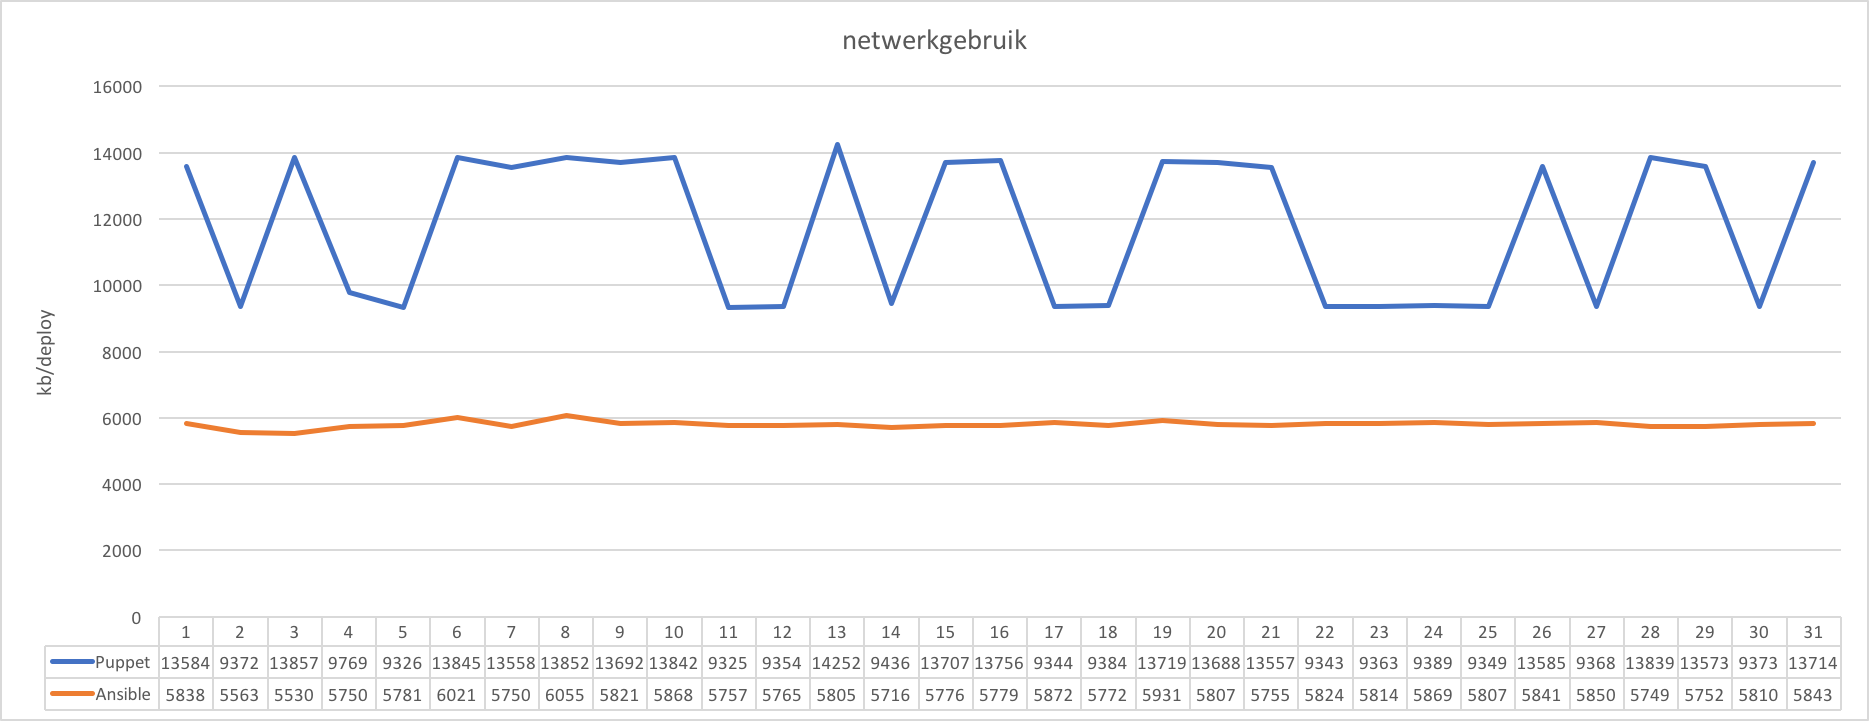
\includegraphics[width=\linewidth]{img/netwerkverbruik.png}
	\caption{Totaal verbruikte netwerkcapaciteit per client gedurende het deployen. Dit bevat enkel communicatie tussen master en client.}  
	\label{fig:netwerkverbruik}
\end{figure}



 %-------------------------------------------------- einde netwerk
 
\subsection{Tijd tot het bekomen van een consistente toestand}

Het is interessant om te weten wat de verhouding is tussen de gemiddelde \gls{configuratietijd} van Ansible en Puppet. Om dit op een zo betrouwbaar mogelijke manier te kunnen verwezenlijken, zijn de configuraties van Ansible en Puppet zo analoog mogelijk gehouden zoals te lezen is in sectie \ref{sec:opstellingtestevn}. De tijd kan worden onderverdeeld in twee delen.\newline
Het eerste deel van de tijd zal de \gls{connectietijd} genoemd worden. Dit is de tijd die het kost alvorens er effectief overgegaan kan worden tot configureren. Hieronder vallen zaken zoals het verzamelen van de nodige configuraties en het verzamelen van server-specifieke waarden (zoals bijvoorbeeld distributie) en het compileren van een catalogus of module. Bij Ansible kon deze tijd gewoon berekend worden op basis van de resultaten\footnote{connectietijd = totaal verstreken tijd -  \unexpanded{$ \sum  $} (tijd playbooks)} dewelke af te lezen zijn van het dashboard dat ge\"integreerd is met Ansible Tower. Bij Puppet is dit echter niet mogelijk en bijgevolg zijn deze resultaten met de hand gemeten.\newline
 De tweede tijd is de \gls{configuratietijd}. Dit is de tijd die nodig is om de configuratie effectief uit te voeren. Deze tijden zijn eenvoudig af te lezen op de uitvoer van de \gls{CMT}'s en het volstaat om deze te noteren.




\subsubsection{\gls{configuratietijd}}

%Aangezien de resultaten van 'volledige configuratie' (zie bijlage C: deploytijden) 
Op afbeelding \ref{fig:deploytime_fullconfig} is geen \'e\'enduidig verschil aan te tonen tussen beide \gls{CMT}'s. Bijgevolg is er met behulp van de Z-toets aangetoond of er al dan niet een statistisch verschil is. Deze berekingen kunnen teruggevonden worden in bijlage A: hypothese configuratietijd.

\begin{figure}
	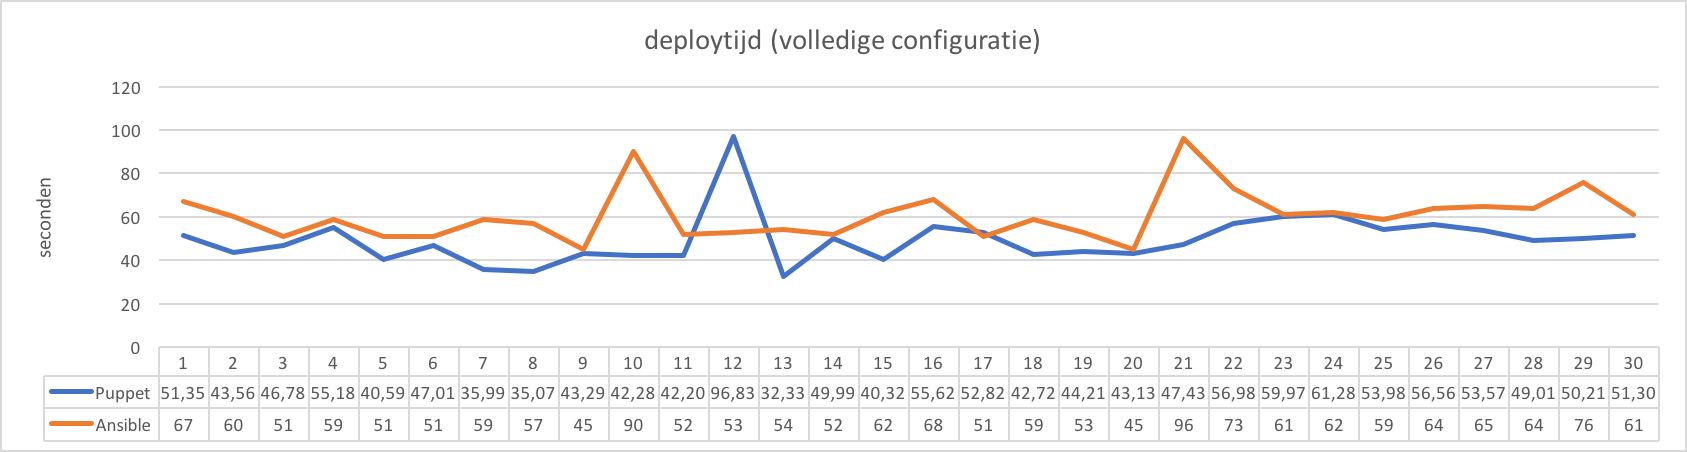
\includegraphics[width=\linewidth]{img/deploytime_fullconfig.png} 
	\caption{Tijd tot het bekomen van een consistente toestand, vertrekkende van een ‘lege' server.}  
	\label{fig:deploytime_fullconfig}
\end{figure}

Hierbij blijkt dat Z buiten het kritisch gebied valt waardoor de nulhypotese verworpen kan worden. Bijgevolg wordt aangenomen dat beide gemiddelden niet tot dezelfde verzameling behoren. Er kan dus worden geconcludeerd dat wanneer er wordt vertrokken van een lege server, Ansible er gemiddeld langer over doet dan Puppet. Dit is in dit geval een verschil van gemiddeld 11,3 seconden. 

De verschillen worden echter nog groter wanneer de test gedaan wordt met een gedeeltelijke configuratie. Hiermee wordt bedoeld dat er vertrokken is van servers die reeds geconfigureerd zijn en er slechts enkele aanpassingen doorgevoerd moeten worden. Deze aanpassingen zijn een service starten en de inhoud van de webpagina veranderen. De resultaten lopen niet door elkaar waardoor een Z-toets niet echt nodig is. Ansible deed gemiddeld 19,10 seconden voor de \gls{deploy} met een vrij grote variatie van 33,40 seconden. Puppet haalde maar een vrij consistente 3,10 seconden met een variatie van 0,35.

In laatste instantie is er gekeken naar de tijd die het zou kosten tot de \gls{CMT} vaststelt dat de server reeds volledig geconfigureerd is en dat er geen aanpassingen meer nodig zijn. Hierbij resulteert Ansible op een gemiddelde van 18 seconden met opnieuw een vrij grote variatie van 18,25 seconden. Ook hier doet Puppet het opnieuw beter aangezien deze minder dan een seconde nodig heeft om vast te stellen dat er geen aanpassingen nodig zijn. Uiteraard zijn al deze waarden afhankelijk van de configuratie maar ze geven wel een duidelijke indicatie van de verschillen tussen beide \gls{CMT}'s.


\begin{figure}
	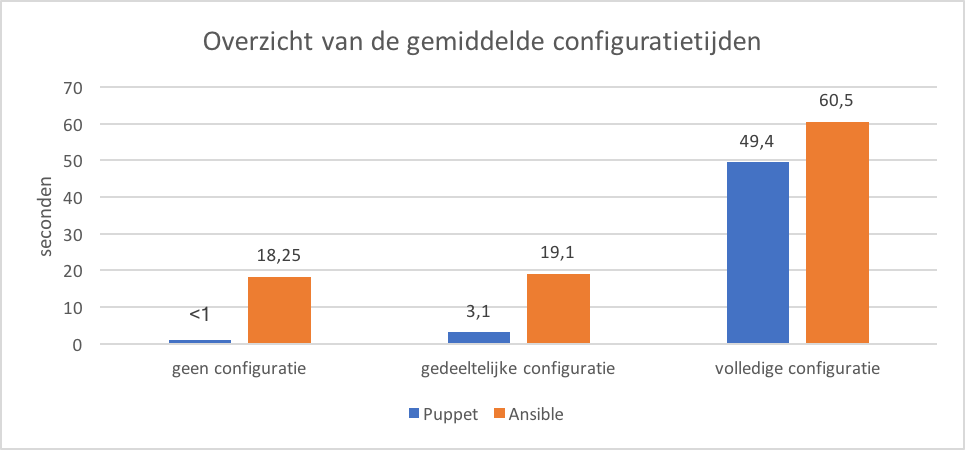
\includegraphics[width=\linewidth]{img/overzichtgemiddeldeconfigtijd.png} 
	\caption{Gemiddelde configuratietijd in seconden.}  

\end{figure}

\textbf{Opmerking:} De \gls{connectietijd} is niet meegerekend in deze metingen. Het omvat hier uitsluitend de \gls{configuratietijd}.

De reden dat Ansible trager is dan Puppet is te wijten aan de manier van communiceren. Puppet verstuurt namelijk een volledige configuratie bij de start. Ansible doet dit niet en verstuurt taak per taak. Hierdoor wordt de verbinding meerdere malen geinitialiseerd en opnieuw verbroken. Deze veronderstelling werd gestaafd door de volgende test:

\begin{addmargin}[2em]{0cm}
\underline{Hypothese A}: Ansible verstuurt taak per taak.\newline
\underline{Hypothese P}: Puppet verstuurt een gehele configuratie op het moment van initialisatie.

\underline{Test}: de verbinding wordt verbroken tijdens het configureren.

\underline{Verwachting A}: nadat de verbinding verbroken is, wordt geen nieuw taak gestart.\newline
\underline{Verwachting P}: de configuratie gaat zonder problemen verder.

\underline{Resultaat A}: de configuratie valt stil. Opmerkelijk hierbij is dat niettemin de configuratie stilvalt, deze niet stopt. De master heeft namelijk niet door dat de verbinding verbroken is en veronderstelt dat de client eenvoudigweg nog bezig is met configureren. Als later de verbinding hersteld wordt, gaat de configuratie opnieuw verder.\newline
\underline{Resultaat P}: de configuratie gaat ongestoord verder.
\end{addmargin}

Bij Ansible wordt er dus per taak, en dus ook per connectie, een module overgebracht van de master naar de client. Deze bestanden zijn terug te vinden in \texttt{$\sim$/.ansible/tmp}. Hierin is duidelijk te zien hoe, tijdens een configuratie, er per taak een nieuwe module (geschreven in Python) verschijnt en vervolgens weer verdwijnt. Dit wordt in dit onderzoek gezien als \'e\'en van de grootste oorzaken waarom Ansible trager is.  \textcite{AnsibleTuning} herkent dit probleem en biedt hiervoor een alternatief aan, genaamd 'pipelinging'. Hierdoor zouden er minder SSH-verbindingen nodig zijn die modules moeten overzetten. Om dit mogelijk te maken moet \texttt{requiretty} uitgezet worden. Meer tips om de performantie te van Ansible te verbeteren kunnen gevonden worden in sectie \ref{sec:schaalbaarheid}.

\subsubsection{Connectietijd}

De \gls{connectietijd} is de periode tussen het moment waarop de opdracht om te configureren gegeven wordt en het moment waarbij er effectief overgegaan kan worden tot configureren. Hieronder vallen zaken zoals het verzamelen van bepaalde gegevens, compileren en het overbrengen van de nodige bestanden en zo verder. Dit fenomeen wordt in dit rapport de \gls{connectietijd} genoemd. Bij de resultaten van de connectietijd is geen duidelijk verschil op te merken. Bovendien liggen de gemiddelden zeer dicht bij elkaar. Om vast te stellen of er een significant verschil is, is er opnieuw gebruik gemaakt van de Z-toets. Deze berekingen kunnen teruggevonden worden in bijlage A, hypothese connectietijd. Z ligt hier echter in het aanvaardingsgebied waardoor de nulhypothese, die stelt dat beide gemiddelden gelijk zijn, aanvaard kunnen worden. Er is bijgevolg geen statistisch verschil tussen beide reeksen.
%\begin{figure}
%  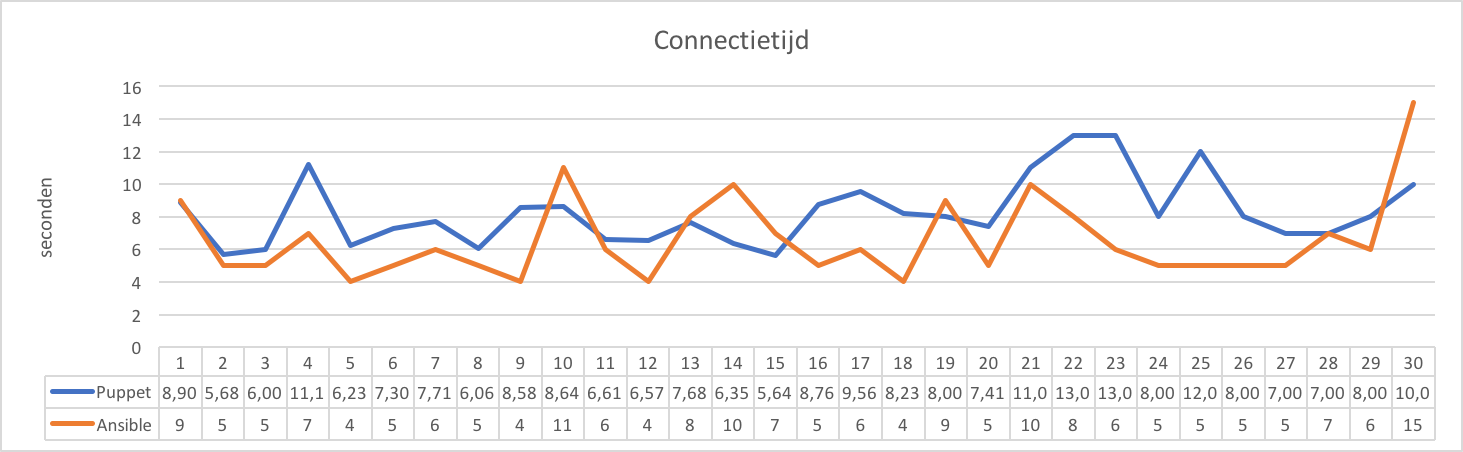
\includegraphics[width=\linewidth]{img/connectiontime.png} 
 % \caption{Tijd tot het initialiseren van een deploy}  
 % \label{fig:connectiontime}
%\end{figure}

\textbf{Er kan hier dus geconcludeerd worden dat Ansible nood heeft aan een voortdurend goede verbinding tussen de master en de client om een snelle configuratie te kunnen verzekeren. Bij Puppet is dit niet nodig aangezien hierbij alle nodige bestanden voor een goede configuratie van meet af aan al aanwezig zijn. Vermoed wordt dat dit \'e\'en van de redenen is waarom Puppet sneller is in configureren.}

 %{\color{red}Volgens deze link zou een reden zijn dat ansible trager is dan puppet omdat ze ssh gebruiken. te onderzoeken. http://www.intigua.com/blog/puppet-vs.-chef-vs.-ansible-vs.-saltstack}



%%---------------------------------------------------- einde performantie


\subsection{Gebruik van het geheugen}

Op grafiek \ref{fig:geheugengebruik} is per tijdseenheid het gemiddeld gebruikt werkgeheugen weergegeven. Hierop is te zien hoe Puppet opvallend meer geheugen gebruikt. Niet alleen tijdens een \gls{deploy} maar ook ervoor en erna. Zelfs wanneer een Ansible client en een Puppet client juist opgezet worden met behulp van Vagrant, is er al een verschil in het gebruikte geheugen. Gezien het feit dat er al een verschil waar te nemen is in deze vroege levensfase van de server en het enige verschil in configuratie op dit moment de Puppetagent is, werd vermoed dat het verschil hier aan te wijten is. Dit vermoeden werd gestaafd toen de Puppetagent tijdelijk uitgezet werd. Het werkgeheugen daalde onmiddellijk naar gelijkwaardige waarden als deze van de Ansibleclient. Zonder configuratie gebruiken Puppetclients gemiddeld 58\% geheugen van de 500MB werkgeheugen. Bij Ansible is dit 47\%. Dit betekent dat met een verschil van 11\%, er bij 500 MB 55MB meer RAM-geheugen gebruikt wordt bij Puppet.

\textbf{Er is dus een duidelijk verschil tussen het geheugengebruik van Puppet clients ten opzichte van Ansible clients. Hierbij gebruikt Puppet dankzij de Puppetagent beduidend meer resources. Ondanks het feit dat een service meer of minder doorgaans niet zorgt voor radicale gevolgen, is de grootste bottleneck nog steeds dat deze service in de eerste plaats ge\"installeerd en geconfigureerd dient te worden. Iets dat niet door Puppet verzorgd kan worden. Bij virtuele servers kan dit opgelost worden door gebruik te maken van een template.}

%{\color{red} Hoe zet \gls{VRT}  momenteel puppetagent op zijn puppetclients? > met template maar hoe bij fysieke server???}


\begin{figure}[hbt!]
  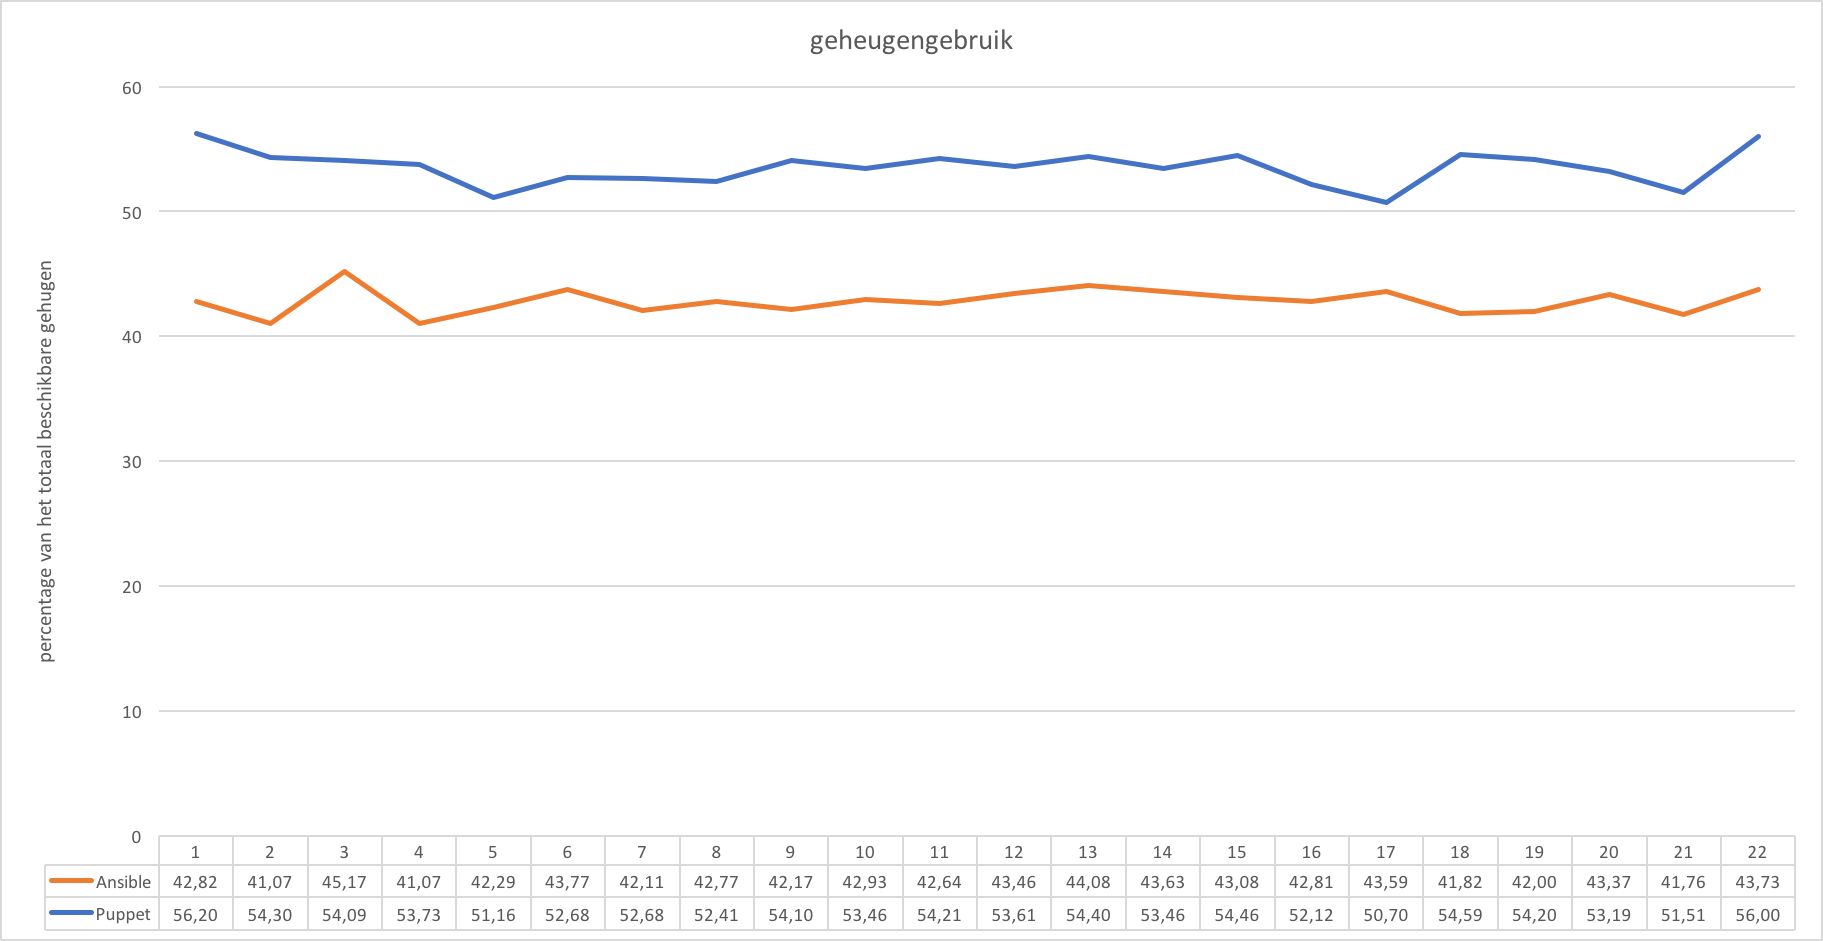
\includegraphics[width=\linewidth]{img/geheugengebruik}
 \caption{Verbruikt percentage van het RAM geheugen. Gemeten bij servers met elk 500 MB. }  
  \label{fig:geheugengebruik}
\end{figure}

%---------------------------------------------
\subsection{Schaalbaarheid}
\label{sec:schaalbaarheid}

Puppet kan minder servers  in parallel behandelen dan Ansible. Dit is ook niet nodig bij Puppet. Eens de Puppetmaster de \gls{catalog} gecompileerd heeft, neemt de Puppetagent die draait op de client het over. Dit is een beduidend kortere doorlooptijd dan Ansible. Aangezien Ansible geen gebruik maakt van deze agents valt niet enkel het compileren onder de verantwoordelijkheid van de master maar ook de uitvoering hiervan. Dit betekent dat Ansible zich over zijn clients moet ontfermen zolang deze hun gewenste consistente toestand niet bereikt hebben.

Puppet heeft buiten de kortere doorlooptijd ook nog het principe van pull-mode dat in zijn voordeel werkt. Aanvragen voor \gls{catalog}sen gebeuren meer verspreid aangezien elke Puppetclient zelf verantwoordelijk is voor zijn updates. De kans dat veel servers tegelijk een aanvraag doen is vrij klein.  Bij Ansible worden vanwege de push-mode wel meerdere servers tegelijk behandeld. Het is dus vanzelfsprekend dat Ansible in staat moet zijn om meerdere configuraties in parallel te behandelen. 




 \subsubsection{Tips om de performantie van Ansible te verbeteren}
 
 Standaard is Ansible geconfigureerd om 5 servers tegelijk te kunnen configureren. Dit aantal kan toenemen door de parameter \texttt{\gls{fork}s} te verhogen naar 100 of zelfs meer. Dit zal inhouden dat Ansible 100 servers op hetzelfde moment kan configureren. Om dit te realiseren is Ansible afhankelijk van het werkgeheugen. Hoe meer werkgeheugen er beschikbaar is, hoe hoger de parameter \texttt{\gls{fork}s} ge\"initialiseerd kunnen worden.
 
Ansible adviseert verder ook om gebruik te maken van \texttt{with\_items} bij het installeren van meerdere packages. Door het gebruik van \texttt{with\_items} zal Ansible deze packages combineren in \'e\'en transactieblok wat de performantie ten goede komt. Zo zou het dus beter zijn om listing \ref{lst:yamltwotask} te structureren zoals listing \ref{lst:yamlonetask}. 


   \lstset{language=clean,caption={Installeer de vereiste onderdelen van PHP in twee delen},label={lst:yamltwotask}}
\begin{lstlisting}[frame=single]

- name: installeer PHP
  package:
    name: php
    state: present

- name: installeer php-mysql
  package:
    name: php-mysqli
    state: present
\end{lstlisting}

  \lstset{language=clean,caption={Installeer de vereiste onderdelen van PHP in \'e\'en keer},label={lst:yamlonetask}}
\begin{lstlisting}[frame=single]
- name: installeer PHP en bijhorende extensies
  package:
    name: {{ item }}
    state: present
  with_items:
    - php
    - php-mysqli
\end{lstlisting}

  Verder beschikt Ansible over een ‘Pull-mode' waarbij elke server zelf instaat voor zijn configuratie. Elke server haalt de code op van een centraal punt en configureert vervolgens zichzelf. Deze manier van werken vereist wel een scriptje op elke server en doet denken aan de werking van Puppet. Een centraal management punt is in deze opstelling echter niet aanwezig en is dus af te raden voor grotere infrastructuren \autocite{AnsibleTuning} .
  
 \subsubsection{Tips om de performantie van Puppet te verbeteren}
 Puppet is door zijn manier van werken ‘van nature' meer geloadbalanced dan Ansible. Toch zijn ook hier een paar zaken die de performantie ten goede komen. Het aantal aanvragen dat Puppet tegelijk kan behandelen is afhankelijk van het aantal cores in de processor dat Puppet ter beschikking krijgt. Wanneer er meer aanvragen zijn dan beschikbare cores zal het overschot aan aanvragen geblokkeerd worden tot er een core weer vrijkomt. Het aantal cores dat Puppet mag gebruiken kan handmatig ingesteld worden met behulp van de parameter \texttt{max active instances}. Wanneer deze naar bijvoorbeeld twee gebracht wordt, zullen twee cores van de processor gebruikt worden, wat tot gevolg heeft dat er ook twee aanvragen tegelijk behandeld kunnen worden. 
 
 Een tweede punt is het verhogen van de \texttt{max heap size} van \gls{JVM}. Door dit te verhogen kan het \ proces meer geheugen opvragen bij het besturingssysteem \autocite{PuppetTuning}.
 
 \textbf{Ondanks het feit dat beide tools mogelijkheden bieden om de performantie te verhogen, blijft Puppet beter geloadbalanced door zijn manier van werken. Ansible zal dus sneller nood hebben aan een upgrade van de hardware dan Puppet. Een voordeel bij Ansible is wel dat het hoofdzakelijk het werkgeheugen is dat een upgrade nodig zal hebben. Dit komt goedkoper uit dan in het geval van Puppet waarbij een CPU met meerdere cores vereist is. }
 

 
 
 \section{Veiligheid}
 \label{sec:veiligheid}
Servers kunnen op allerlei manieren  corrupt worden. Malafide personen kunnen binnendringen en bestanden aanpassen met als doel bijvoorbeeld een firewall uitschakelen. Weliswaar hoeft het niet altijd zo drastisch te verlopen. Soms worden servers in een inconsistente toestant gebracht door intern personeel dat goedbedoeld updates wilt doorvoeren met onvoorziene nadelige consequenties tot gevolg.
Een \gls{CMT} kan hier een oplossing bieden.  Aangezien een goed geconfigureerde \gls{CMT} op regelmatige basis de nodige servers controleert, kunnen snel mogelijke gevaren vastgesteld en opgelost worden. Stel bijvoorbeeld dat een verkeerde gebruikersgroep toegang heeft gekregen tot een belangrijke productieserver door een menselijke fout. Wanneer eventjes later de \gls{CMT} de client zijn configuratie nakijkt, zal deze vaststellen dat de gebruikersgroepen niet meer in orde zijn en zal deze aanpassen \footnote{Het kan weliswaar gebeuren dat deze aanpassingen terecht zijn en dat de configuratie van de \gls{CMT} verouderd is. Daarom zal de \gls{VRT} Ansible playbooks laten draaien in check-modus. Hiebij controleert hij de server maar voert geen aanpassingen door.}. 

Normaal komen veiligheidsproblemen pas heel laat aan het licht en meestal zelfs pas als het al te laat is. Dankzij een \gls{CMT} kan dit in belangrijke mate gereduceerd worden. Belangrijk hierbij is dat de rapporten die de \gls{CMT} genereert op regelmatige basis gecontroleerd worden.  Wanneer een belangrijke configuratie om een verkeerde manier aangepast is geweest, moet misschien de oorzaak van deze wijziging onderzocht worden om dit in de toekomst te kunnen voorkomen.

Een goede beveiliging van de Puppetmaster of Ansible Tower is van het allergrootst belang. Dit omdat deze server toegang heeft tot verschillende andere servers. Wanneer een ‘gewone' server in verkeerde handen valt, kan dit vanzelfsprekend tot verregaande gevolgen leiden maar de impact op andere servers blijft beperkt. Wanneer dit echter de Ansible- of Puppetmaster betreft, is de impact veel groter. Deze master heeft niet enkel toegang tot vele andere servers maar doorgaans ook belangrijke rechten om de nodige zaken te kunnen configureren.

Bij grotere bedrijven worden Ansible rollen en Puppet modules doorgaans bewaard op daarvoor bestemde servers bedoeld voor source control. Ook voor deze server in het van belang dat personen enkel toegang krijgen tot specifieke rollen en modules. Zo moet de databankbeheerder enkel toegang krijgen tot code die zijn databanken configureren terwijl dat voor andere personen weer andere rollen en modules zullen zijn. Het is dus van belang dat de correcte rechten worden toegepast op deze source control servers.

Zowel Ansible als Puppet schenken de nodige aandacht om zo veilig mogelijk te werk te gaan. Beiden gebruiken encryptie in hun vorm van communiceren. Puppet maakt hierbij gebruik van HTTPS terwijl dit bij Ansible via SSH geregeld wordt. Verder moet bij Puppet elke server handmatig geautoriseerd worden alvorens deze configuraties bij de master kan aanvragen. Bij Ansible is dit niet nodig. Hij bepaalt zelf welke servers hij wenst te configureren. Weliswaar dient hij toegang te krijgen tot elk van deze servers. Het is dus niet mogelijk om met een ongeauthoriseerde server configuraties te ontfutselen bij de master en de client op deze wijze door te laten gaan als legitiem. 

Of Ansible veiliger is dan Puppet is moeilijk te bewijzen. Er zijn wel enkele aanwijzingen die stellen dat Ansible een voordeel heeft op gebied van veiligheid. Zo dient bij Puppet poort 8140 voortdurend open te staan om aanvragen te behandelen. Bij Ansible worden deze configuraties gestart door de master zelf. Hierbij moet wel poort 22 (SSH) open staan op elke client, maar dit is doorgaans sowieso al van toepassing. Bovendien heeft Ansible geen daemon zoals Puppet die op rootlevel geïnstalleerd moet worden.



 %---------------------------------------------------------------------------------------------------------------------------------------------------------------------------------------------------------------------------------------------------------------------------------------------------------------------------------------------------------------------------------------------------------------------------------------------------------------------------------------------------------------------------------------------------------------------------------------------------------------------------------------------------------------------------------------------------------------------------------------------------------------------------------------------------------------------------------------------------------------------------------------------------------------------------------------------------------------------------------------------------------------------------------------------------------------------------------------------------------%
\section{Wat is het verloop van een transitperiode?}
\label{sec:methodologie-verloop-transit}
\subsection{Een geleidelijke overgang}


\begin{wrapfigure}{R}{0.4\textwidth}
\centering
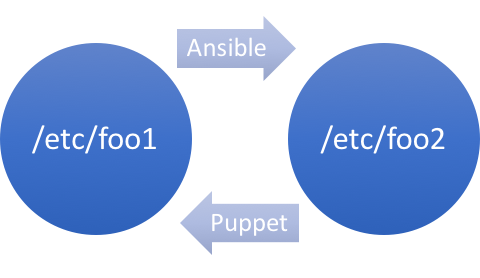
\includegraphics[width=0.4\textwidth]{img/vicieuzecirkel.PNG}
\caption{\label{fig:vicieuzecirkel}Vicieuze cirkel van twee \gls{CMT}'s die hetzelfde bestand proberen te configureren.}
\end{wrapfigure}

De manier waarop Ansible het best ge\"integreerd kan worden verschilt van bedrijf tot bedrijf. In het geval van de \gls{VRT} verloopt dit vlot. \textbf{Ansible en Puppet kunnen namelijk perfect naast elkaar in dezelfde infrastructuur bestaan.} Dit is ideaal voor een geleidelijke en gefaseerde overgang die bij de \gls{VRT} de voorkeur geniet boven een `big bang' scenario. Hierdoor worden risico's ingeperkt en past het beter bij een cultuur gebasseerd op `agile' principes waarbij getracht wordt veranderingen te spreiden in kleinere interatieve stappen. 

E\'en en dezelfde server kan bovendien geconfigureerd worden door zowel Puppet als Ansible. Dit heeft als voordeel dat niet alle modules geschreven in Puppet onmiddellijk vertaald hoeven te worden naar Ansible. Enkele rollen kunnen geschreven zijn voor Ansible terwijl een ander deel nog onder de bevoegdheid van Puppet valt.

 Belangrijk hierbij is wel dat Puppet en Ansible verschillende configuraties dienen te behandelen. Wanneer beide \gls{CMT}'s eenzelfde configuratie uitvoeren, kan er door subtiele verschillen een vicieuze cirkel ontstaan.
Veronderstel een situatie zoals in figuur \ref{fig:vicieuzecirkel}. In Ansible staat een bestand met een extra spatie, hier wordt deze voor de gelegenheid 'foo1' genoemd. Bij Puppet staat deze extra spatie er niet, deze wordt 'foo2' genoemd. 
\begin{enumerate}
\item Puppet configureert de service met bestand foo1 en start deze op.
\item  Eventjes later stelt Ansible vast dat de configuratie niet meer overeenkomt met deze beschreven in het playbook. Hij wijzigt foo1 naar foo2 en herstart de service zodat aanpassingen doorgevoerd zouden worden.
\item  Op een later ogenblik zal Puppet dit waarnemen en het bestand terugdraaien naar foo1, opnieuw gevolgd door een gestart van de gerelateerde service.
\end{enumerate}
Het is vanzelfsprekend dat dit voor onnodige aanpassingen zorgt met eventueel ongewenste of onverwachte gevolgen zoals het voortdurend herstarten van een service.

In de testopstelling is gekeken geweest naar het gedrag van beide \gls{CMT}'s wanneer deze op hetzelfde moment dezelfde server trachten te configureren. Dit veroorzaakte geen problemen.
Het enigste wat dit als nadelig gevolg kan hebben, is dat de configuratie langer duurt dan normaal. Wanneer \gls{CMT} A een lock heeft op de \gls{packagemanager}, dan zal \gls{CMT} B moeten wachten tot deze vrij komt. 

\subsection{Implementatie van Ansible}
In eerste instantie moet Ansible beschikken over een overzicht van alle servers. In de omgeving van de \gls{VRT} maakt Puppet gebruik van \gls{LDAP}. Hieruit kan hij de nodige variabelen ophalen. Vervolgens configureert Puppet de servers met deze waarden. Ideaal is dat de nieuwe Ansible integratie zo analoog mogelijk is aan de huidige manier van werken. Om de waarden op te kunnen halen uit \gls{LDAP} voorziet Ansible Tower geen standaard functionaliteit. Dit wordt opgevangen door gebruik te maken van een script. Hierbij dient Ansible twee methodes op te roepen. Een eerste voor het populeren van groepen en hosts en een tweede voor het toevoegen van variabelen voor elk van deze hosts. Ansible Tower verwacht dat deze methodes JSON retourneren. Op deze wijze kan Ansible dynamisch een inventaris maken van alle servers die onder zijn verantwoordelijkheid vallen.

In tweede instantie moet Ansible de juiste playbooks op kunnen halen. Hiervoor dient de source control server correct ingesteld te staan. Niet alleen op gebied van rechten zoals aangehaald in sectie \ref{sec:veiligheid}, maar ook op gebied van configuratie. Aangezien servers in productie niet dezelfde configuratie mogen hebben als servers in staging moet een duidelijk onderscheid gemaakt worden. Dit kan verwezenlijkt worden door gebruik te maken van \gls{Git-branch}ing. Vervolgens wordt elke branch gekoppeld met de corresponderende groep servers uit de inventaris die worden gegenereerd zoals beschreven in voorgaande alinea. Om hierbij aan een goed versiebeheer te kunnen doen, wordt elke Ansible rol in \gls{Git} toegevoegd als een \gls{submodule}. Elke commit gaat gepaard met een versienummer. Dit stelt de gebruikers in staat om eenvoudig een roll-back te doen in het geval dat bepaalde updates zouden mislukken.

Eens de inventories aangemaakt worden en de source code opgehaald is geweest is het de taak van  Ansible Tower om deze twee te combineren en uit te voeren op de servers. Hiervoor dient hij uiteraard toegang te krijgen tot de desbetreffende servers.

%\subsection{Doel van Ansible Tower}
%Overschakelen naar Ansible Tower houdt automatisch in dat er wordt overgeschakeld naar de commerci\"ele versie van Ansible. Indien er getwijfeld wordt of Ansible Tower een meerwaarde biedt aan de infrastructuur wordt er best rekening gehouden met de volgende zaken. Ansible Tower biedt pas een meerwaarde in grotere omgevingen. 




%---------------------------------------------------------------------------------------------------------------------------------------------------------------------------------------------------------------------------------------------------------------------------------------------------------------------------------------------------------------------------------------------------------------------------------------------------------------------------------------------------------------------------------------------------------------        prijskaartje ----------------------------------------------------------------------------------------------------------------------------------------------------------------------------------------------------------------------------------------------------------------------------------------------------------------------------------------------------------------------------------------------------------------------------------------------------------------------------------------------------------%
 \section{Prijskaartje}

Ansible heeft een ander revenue model dan Puppet. Voor standaard enterprise support rekent \textcite{ansibleprice} 9.092,15 euro voor 100 nodes. \textcite{puppetprice} berekent de prijst op het aantal gebruikte nodes. Dit is dan 109,12 euro per node. Bij 100 nodes komt Puppet dus duurder uit. Zijn er echter minder als 100 nodes, dan is Ansible duurder want er wordt voor exact 100 nodes betaald. Bij meerdere nodes dient een offerte aangevraagd te worden. Ook voor de premium editie dient voor beide technologie\"en een offerte aangevraagd te worden. \footnote{De prijzen omgerekend van USD naar EUR tegen de wisselkoers van 5/5/2017}

